\section{一元变换}
\label{sec:rvt-univariate}

设$X$有密度$f_X$，$g$是实轴上的函数，$Y=g(X)$。$Y$有没有密度？有的话怎样从$f_X$算出来？离散的情形已经由式~\eqref{eq:rvt-discrete-pushforward}解决，难点在连续的情形。

\paragraph{先求分布函数}
最稳妥的办法分两步。第一步取阈值事件$\{Y\leq y\}$，写出它的原像，用式~\eqref{eq:rvt-cdf-method}求出$F_Y(y)$；这一步对任何$g$都适用。第二步在$F_Y$可导的地方求导得到密度，这一步需要条件，后面两小节说明。这种做法称为\term{分布函数法}（distribution function method）。

以$X\sim\operatorname{Unif}(0,1)$、$Y=X^2$为例。$Y$取值于$(0,1)$。对$0<y<1$，$X^2\leq y$与$X\leq\sqrt{y}$等价，因为$X$只取正值，于是
\[
 F_Y(y)=\mathbb{P}(X\leq\sqrt{y})=\sqrt{y} .
\]
$y\leq0$时$F_Y(y)=0$，$y\geq1$时$F_Y(y)=1$。在$(0,1)$内求导，得到
\[
 f_Y(y)=\frac{1}{2\sqrt{y}},\qquad 0<y<1 .
\]

$X$的密度在$(0,1)$上处处是$1$，$Y$的密度却在$0$附近无界。原因是平方把$0$附近的数压得更挤：$X\in(0,0.1)$的概率是$0.1$，被送进长度只有$0.01$的区间$(0,0.01)$，单位长度上的质量变成$10$倍。

图~\ref{fig:rvt-preimage-cdf}画出阈值事件的原像。在$(0,1)$上，$X^2\leq y$的原像是一段从$0$开始的区间；如果$X$也取负值，比如$X\sim\operatorname{Unif}(-1,2)$，原像就变成$[-\sqrt{y},\sqrt{y}]$与支撑的交，两个端点同时移动。前者是单调变换，后者是多分支变换，分别在下面两小节处理。

\begin{BookInlineFigure}
  \centering
  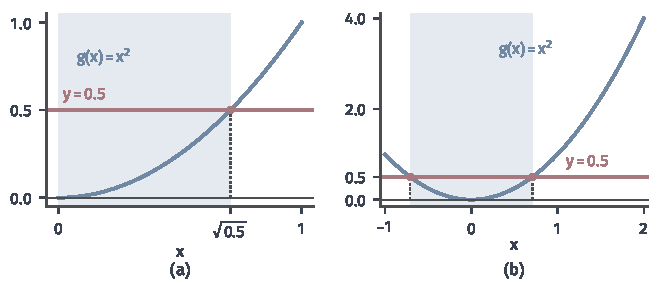
\includegraphics[width=112mm]{figures/07-probability/01-elementary-probability/matplotlib/rvt-preimage-cdf/figure.pdf}
  \caption{阈值事件的原像。蓝线是$g(x)=x^2$，红色水平线是阈值$y=0.5$，横轴上的浅蓝区间是$\{x:\ x^2\leq0.5\}$与$X$的支撑之交。(a)$X$取值于$(0,1)$，原像是$(0,\sqrt{0.5}\,]$；(b)$X$取值于$(-1,2)$，原像是$[-\sqrt{0.5},\sqrt{0.5}\,]$，左右两端都随$y$移动。}
  \label{fig:rvt-preimage-cdf}
\end{BookInlineFigure}

\subsection{单调变换}
\label{sec:rvt-monotone}

上面的计算每次都要从分布函数重新开始。对单调的$g$，这两步可以合成一个公式，并且看清密度为什么要乘以一个伸缩因子。

\paragraph{阈值事件的翻译}
设$g$在$X$的取值区间上严格递增，反函数为$h$。$g(X)\leq y$与$X\leq h(y)$等价，于是
\[
 F_Y(y)=F_X\bigl(h(y)\bigr) .
\]
$g$严格递减时，不等号要翻转：$g(X)\leq y$与$X\geq h(y)$等价。$X$有密度，单点的概率为零，于是
\[
 F_Y(y)=\mathbb{P}\bigl(X\geq h(y)\bigr)=1-F_X\bigl(h(y)\bigr) .
\]

\paragraph{长度的伸缩}
求导之前先看密度应当变成什么。$X$落在$[x,x+\Delta x]$的概率约为$f_X(x)\Delta x$。$g$把这段区间送到以$g(x)$为一端、长度约$\lvert g'(x)\rvert\Delta x$的区间，概率不变，长度乘了$\lvert g'(x)\rvert$，所以单位长度上的质量要除以$\lvert g'(x)\rvert$。这就得到下面的公式，导数取绝对值，因为长度总是正的。

\begin{theorem}[单调变换的密度]
\label{thm:rvt-monotone-density}
设$X$的密度$f_X$在开区间$I$之外为零（$I$可以无界），$g$在$I$上严格单调、连续可导，且对所有$x\in I$有$g'(x)\neq0$。记$J=g(I)$，$h:J\to I$为$g$的反函数。则$Y=g(X)$有密度
\begin{equation}
 f_Y(y)=
 \begin{cases}
  f_X\bigl(h(y)\bigr)\,\lvert h'(y)\rvert, & y\in J,\\
  0, & y\notin J .
 \end{cases}
 \label{eq:rvt-monotone-density}
\end{equation}
其中$h'(y)=1/g'(h(y))$。
\end{theorem}

\begin{proof}
由一元反函数的求导法则，$h$在开区间$J$上连续可导，且$h'(y)=1/g'(h(y))$。只需证明对$J$内任意闭区间$[c,d]$，$\mathbb{P}(c\leq Y\leq d)$等于式~\eqref{eq:rvt-monotone-density}在$[c,d]$上的积分；区间概率确定了分布函数，也就确定了分布。

先设$g$递增，此时$h$也递增，$h'>0$。原像规则给出
\[
 \mathbb{P}(c\leq Y\leq d)=\mathbb{P}\bigl(h(c)\leq X\leq h(d)\bigr)=\int_{h(c)}^{h(d)}f_X(x)\,\mathrm{d}x .
\]
作换元$x=h(y)$，$\mathrm{d}x=h'(y)\,\mathrm{d}y$，积分限$h(c),h(d)$对应$c,d$，得到
\[
 \int_{h(c)}^{h(d)}f_X(x)\,\mathrm{d}x=\int_c^d f_X\bigl(h(y)\bigr)\,h'(y)\,\mathrm{d}y .
\]
这里$h'=\lvert h'\rvert$，就是要证的等式。

再设$g$递减，此时$h$递减，$h'<0$，原像变成$[h(d),h(c)]$。同样的换元给出
\[
 \int_{h(d)}^{h(c)}f_X(x)\,\mathrm{d}x=\int_d^c f_X\bigl(h(y)\bigr)\,h'(y)\,\mathrm{d}y=\int_c^d f_X\bigl(h(y)\bigr)\bigl(-h'(y)\bigr)\,\mathrm{d}y .
\]
交换积分限产生的负号与$h'<0$抵消，被积函数仍是$f_X(h(y))\lvert h'(y)\rvert$。

$J$外的区间原像为空，概率为零。$I$无界或$f_X$在端点附近无界时，上面的积分是反常积分，先在内部的闭区间上换元，再令端点趋于边界即可。
\end{proof}

换元积分的依据见\BookChapterRef{chap:univariate-integration}{卷一第7章“一元函数的积分”}。证明中递减情形的处理正好对应前面的两件事：阈值事件的不等号翻转，表现为积分限交换；长度为正，表现为导数取绝对值。

条件各有作用。严格单调保证每个$y$只有一个逆像，原像是一段区间。$g'\neq0$保证小区间不会被压成一个点；它一旦在某段区间上失效，就会产生原子。连续可导是换元公式所需的光滑性。最后，$J=g(I)$交代了输出的支撑，式~\eqref{eq:rvt-monotone-density}在$J$外必须补成零。

\paragraph{线性变换}
$Y=aX+b$，$a\neq0$。反函数$h(y)=(y-b)/a$，$\lvert h'(y)\rvert=1/\lvert a\rvert$，于是
\begin{equation}
 f_Y(y)=\frac{1}{\lvert a\rvert}\,f_X\Bigl(\frac{y-b}{a}\Bigr) .
 \label{eq:rvt-linear-density}
\end{equation}
$a>0$时密度的形状被横向拉伸$a$倍、纵向压低$a$倍，再平移$b$；$a<0$时还要左右翻转。

两个具体情形。$X\sim\mathcal{N}(\mu,\sigma^{2})$时，代入密度并整理指数，得到
\[
 f_Y(y)=\frac{1}{\sqrt{2\pi}\,\lvert a\rvert\sigma}\exp\Bigl(-\frac{(y-a\mu-b)^2}{2a^2\sigma^2}\Bigr),
\]
即$Y\sim\mathcal{N}(a\mu+b,a^2\sigma^2)$，高斯族在仿射变换下保持不变。$X\sim\operatorname{Unif}(0,1)$、$Y=3-2X$时，$a=-2$，$Y$的支撑是$(1,3)$，密度为$1/2$；支撑的端点由$I=(0,1)$的端点经$g$映过去，次序也翻转了。

\paragraph{指数变换}
设$X\sim\mathcal{N}(\mu,\sigma^{2})$，$Y=\mathrm{e}^{X}$。$g(x)=\mathrm{e}^{x}$把$I=\mathbb{R}$映到$J=(0,\infty)$，反函数$h(y)=\ln y$，$h'(y)=1/y$。代入式~\eqref{eq:rvt-monotone-density}，得到
\begin{equation}
 f_Y(y)=\frac{1}{y\,\sigma\sqrt{2\pi}}\exp\Bigl(-\frac{(\ln y-\mu)^2}{2\sigma^2}\Bigr),\qquad y>0 .
 \label{eq:rvt-lognormal}
\end{equation}
这个分布称为\term{对数正态分布}（log-normal distribution）：取对数之后服从高斯分布。输出只取正值，这来自$g$的值域，而不是来自$X$的密度。

图~\ref{fig:rvt-lognormal-strip}取$\mu=0$、$\sigma=1$，把$X$的一条小区间$[0.5,0.7]$和它的像$[\mathrm{e}^{0.5},\mathrm{e}^{0.7}]\approx[1.649,2.014]$画在一起。两块浅蓝面积都等于$\Phi(0.7)-\Phi(0.5)\approx0.0666$，其中$\Phi$是标准高斯分布函数。像区间的长度约$0.365$，比原来的$0.2$长，所以那里的密度相应变低。

\begin{BookInlineFigure}
  \centering
  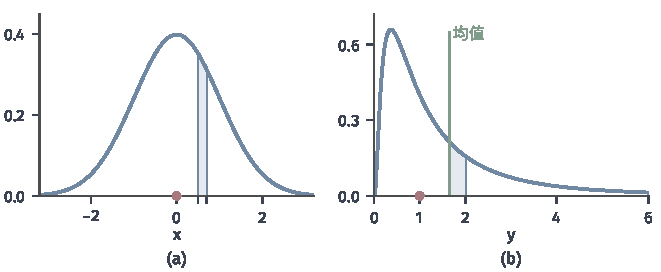
\includegraphics[width=112mm]{figures/07-probability/01-elementary-probability/matplotlib/rvt-lognormal-strip/figure.pdf}
  \caption{指数变换下质量守恒、长度伸缩。(a)$X\sim\mathcal{N}(0,1)$的密度，浅蓝区间为$[0.5,0.7]$；(b)$Y=\mathrm{e}^{X}$的对数正态密度，浅蓝区间为像$[\mathrm{e}^{0.5},\mathrm{e}^{0.7}]$，两块面积都约为$0.0666$。红点标出中位数：$X$的中位数$0$对应$Y$的中位数$1$；绿色竖线是$Y$的均值$\mathrm{e}^{1/2}$。}
  \label{fig:rvt-lognormal-strip}
\end{BookInlineFigure}

单调变换保持分位数：$X$的中位数是$0$，$\mathrm{e}^{X}\leq\mathrm{e}^{0}$与$X\leq0$等价，所以$Y$的中位数是$\mathrm{e}^{0}=1$。均值却不这样传递。按第~\ref{chap:random-variable-moments}章的函数期望，对指数配方，得到
\[
 \mathbb{E}[\mathrm{e}^{X}]=\int_{\mathbb{R}}\frac{\mathrm{e}^{x}}{\sqrt{2\pi}\sigma}\mathrm{e}^{-(x-\mu)^2/(2\sigma^2)}\,\mathrm{d}x=\mathrm{e}^{\mu+\sigma^2/2} .
\]
$\mu=0$、$\sigma=1$时均值约为$1.649$，大于$\mathrm{e}^{\mathbb{E}[X]}=1$。这与Jensen不等式一致：$\mathrm{e}^{x}$是凸函数，先平均再变换小于先变换再平均。

\paragraph{递减的情形}
设$X\sim\operatorname{Exp}(\lambda)$，$Y=\mathrm{e}^{-X}$。$g$把$(0,\infty)$递减地映到$(0,1)$，反函数$h(y)=-\ln y$。先用阈值事件：对$0<y<1$，$\mathrm{e}^{-X}\leq y$与$X\geq-\ln y$等价，不等号翻转了，于是
\[
 F_Y(y)=\mathbb{P}(X\geq-\ln y)=\mathrm{e}^{-\lambda(-\ln y)}=y^{\lambda} .
\]

再用式~\eqref{eq:rvt-monotone-density}核对。$h'(y)=-1/y$，取绝对值得$1/y$；密度在逆像处的值是
\[
 f_X\bigl(h(y)\bigr)=\lambda\mathrm{e}^{\lambda\ln y}=\lambda y^{\lambda} .
\]
两者相乘，得到
\[
 f_Y(y)=\lambda y^{\lambda}\cdot\frac{1}{y}=\lambda y^{\lambda-1},\qquad 0<y<1 ,
\]
正是$F_Y(y)=y^{\lambda}$的导数。$\lambda=1$时$Y\sim\operatorname{Unif}(0,1)$；反过来读，$U\sim\operatorname{Unif}(0,1)$时$-\ln U\sim\operatorname{Exp}(1)$。

递减情形有两处容易出错，图~\ref{fig:rvt-decreasing-map}取$\lambda=2$画出正确结果。若忘了翻转不等号，会写出$F_Y(y)=1-y^{2}$，它随$y$递减，不可能是分布函数。若忘了绝对值，会得到“密度”$-2y$，它是负的。两个检查——分布函数递增、密度非负——可以随手做。

\begin{BookInlineFigure}
  \centering
  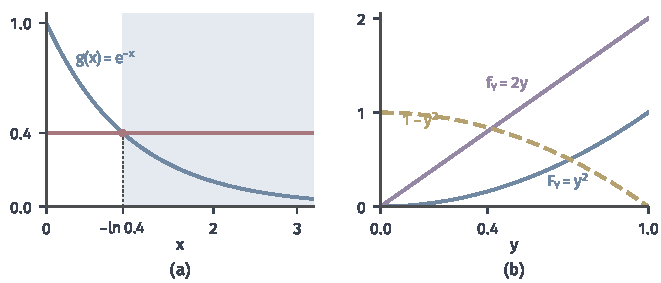
\includegraphics[width=112mm]{figures/07-probability/01-elementary-probability/matplotlib/rvt-decreasing-map/figure.pdf}
  \caption{递减变换$Y=\mathrm{e}^{-X}$，$X\sim\operatorname{Exp}(2)$。(a)蓝线为$g(x)=\mathrm{e}^{-x}$，红线为阈值$y=0.4$，事件$Y\leq0.4$的原像是横轴上的右侧区间$[-\ln0.4,\infty)$（浅蓝）。(b)$Y$的分布函数$y^{2}$（蓝）与密度$2y$（紫），黄色虚线是不翻转不等号得到的$1-y^{2}$，它不是分布函数。}
  \label{fig:rvt-decreasing-map}
\end{BookInlineFigure}

\paragraph{非退化条件失效}
条件$g'\neq0$去掉会怎样，要分两种情况看。第一种是$g$在一段区间上为常数。取$X\sim\operatorname{Unif}(0,2)$，$Y=\min(X,1)$。$X\in[1,2)$的全部质量都被送到点$1$，于是
\[
 \mathbb{P}(Y=1)=\mathbb{P}(X\geq1)=\frac12 .
\]
$Y$的分布函数在$1$处跳跃$1/2$，没有密度。若只在$(0,1)$上套用式~\eqref{eq:rvt-monotone-density}，得到的函数是$1/2$，总积分只有$1/2$，另一半质量丢在了原子上。

第二种是$g'$只在孤立点为零。取$X\sim\operatorname{Unif}(-1,1)$，$Y=X^3$，$g'(0)=0$。去掉单点$0$，把$I$分成$(-1,0)$与$(0,1)$，每段上定理的条件都成立；单点的概率为零，不影响结果。两段的反函数都是$h(y)=y^{1/3}$，在$y\neq0$处$\lvert h'(y)\rvert=\tfrac13\lvert y\rvert^{-2/3}$，于是
\[
 f_Y(y)=\frac12\cdot\frac{1}{3\lvert y\rvert^{2/3}}=\frac{1}{6\lvert y\rvert^{2/3}},\qquad 0<\lvert y\rvert<1 .
\]
它在$0$附近无界，但可积，总积分为$2\cdot\tfrac16\cdot3=1$。

图~\ref{fig:rvt-flat-atom}对比两种情况。导数在一段区间上为零，会把正长度的区间压成一个点，产生原子；只在一个点上为零，压缩的是零概率的点，密度变得无界，但仍然存在。

\begin{BookInlineFigure}
  \centering
  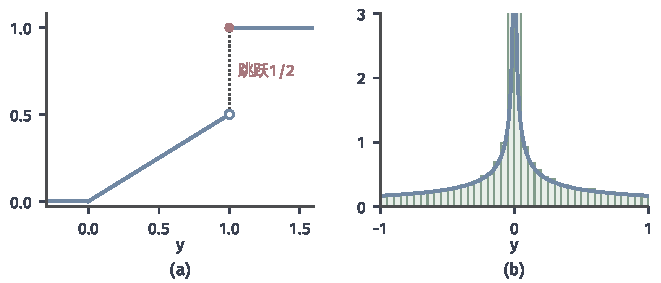
\includegraphics[width=112mm]{figures/07-probability/01-elementary-probability/matplotlib/rvt-flat-atom/figure.pdf}
  \caption{导数为零的两种后果。(a)$Y=\min(X,1)$，$X\sim\operatorname{Unif}(0,2)$，分布函数（蓝）在$y=1$处跳跃$1/2$，红点表示该原子。(b)$Y=X^3$，$X\sim\operatorname{Unif}(-1,1)$，密度$\tfrac16\lvert y\rvert^{-2/3}$（蓝）在$0$附近无界，浅绿直方图是$20000$个模拟样本（种子$7$）。}
  \label{fig:rvt-flat-atom}
\end{BookInlineFigure}

\subsection{多分支变换}
\label{sec:rvt-branches}

$g$不单调时，一个$y$可以有几个逆像。图~\ref{fig:rvt-preimage-cdf}(b)中，$X\sim\operatorname{Unif}(-1,2)$，$y=0.5$有两个逆像$\pm\sqrt{0.5}$，而$y=2$只有一个逆像$\sqrt2$，因为$-\sqrt2$在支撑之外。要把每个逆像附近的质量都收集起来。

\paragraph{分支相加}
做法是把输入区域切成几段，每段上$g$单调，在每段上用单调变换的公式，再把各段的贡献相加。用质量的图景说，输出$y$附近的质量来自几处输入，每处按自己的伸缩比例换算后叠在一起。

\begin{theorem}[多分支变换的密度]
\label{thm:rvt-branch-density}
设$X$的密度在$I_1\cup\cdots\cup I_m$之外为零，其中$I_1,\ldots,I_m$是互不相交的开区间（除去有限个点后覆盖$X$的取值范围）。设$g$在每个$I_k$上满足定理~\ref{thm:rvt-monotone-density}的条件，$h_k$是$g$在$I_k$上的反函数，定义在$J_k=g(I_k)$上。则$Y=g(X)$有密度
\begin{equation}
 f_Y(y)=\sum_{k:\ y\in J_k}f_X\bigl(h_k(y)\bigr)\,\lvert h_k'(y)\rvert .
 \label{eq:rvt-branch-density}
\end{equation}
\end{theorem}

\begin{proof}
对任意区间$[c,d]$，事件$c\leq Y\leq d$按$X$落在哪一段分解为互不相交的事件之并，剩下的有限个点概率为零：
\[
 \mathbb{P}(c\leq Y\leq d)=\sum_{k=1}^{m}\mathbb{P}\bigl(X\in I_k,\ c\leq g(X)\leq d\bigr) .
\]
第$k$项等于$f_X\mathbf{1}_{I_k}$在$I_k\cap g^{-1}([c,d])$上的积分。定理~\ref{thm:rvt-monotone-density}的证明只用到换元积分，没有用到总质量为$1$，所以对$f_X\mathbf{1}_{I_k}$同样成立，第$k$项等于$f_X(h_k(y))\lvert h_k'(y)\rvert$在$[c,d]\cap J_k$上的积分。对$k$求和，得到式~\eqref{eq:rvt-branch-density}在$[c,d]$上的积分。
\end{proof}

\paragraph{平方变换}
设$Z\sim\mathcal{N}(0,1)$，$Y=Z^2$。两段$I_1=(-\infty,0)$、$I_2=(0,\infty)$都被映到$(0,\infty)$，反函数$h_{1,2}(y)=\mp\sqrt{y}$，$\lvert h_k'(y)\rvert=1/(2\sqrt{y})$。记标准高斯密度为$\varphi(z)=\mathrm{e}^{-z^2/2}/\sqrt{2\pi}$，它是偶函数，两项相等，于是
\begin{equation}
 f_Y(y)=2\cdot\varphi(\sqrt{y})\cdot\frac{1}{2\sqrt{y}}=\frac{1}{\sqrt{2\pi}}\,y^{-1/2}\mathrm{e}^{-y/2},\qquad y>0 .
 \label{eq:rvt-chi2-one}
\end{equation}
与第~\ref{chap:common-distributions}章的Gamma密度比较，这正是$\operatorname{Gamma}(1/2,1/2)$，即自由度为$1$的$\chi^2$分布：标准高斯的平方服从$\chi^2_1$。只取$h_2(y)=\sqrt{y}$一支，得到的函数总积分为$1/2$，漏掉了$Z<0$的一半。

支撑不对称时，各段的像可以不同。$X\sim\operatorname{Unif}(-1,2)$，密度$1/3$，$Y=X^2$取值于$(0,4)$。$I_1=(-1,0)$映到$J_1=(0,1)$，$I_2=(0,2)$映到$J_2=(0,4)$。$0<y<1$时两支都有贡献，$1<y<4$时只有右支，于是
\[
 f_Y(y)=
 \begin{cases}
  \dfrac13\cdot\dfrac{1}{2\sqrt{y}}\cdot2=\dfrac{1}{3\sqrt{y}}, & 0<y<1,\\
  \dfrac13\cdot\dfrac{1}{2\sqrt{y}}=\dfrac{1}{6\sqrt{y}}, & 1<y<4 .
 \end{cases}
\]

两段的质量分别是
\[
 \int_0^1\frac{\mathrm{d}y}{3\sqrt{y}}=\frac23,\qquad \int_1^4\frac{\mathrm{d}y}{6\sqrt{y}}=\frac13 .
\]
合计为$1$。第一段的$2/3$也可以直接核对：$Y<1$等价于$-1<X<1$，概率是$2/3$。图~\ref{fig:rvt-square-branches}显示密度在$y=1$处减半，这是左支走到尽头的位置。

\begin{BookInlineFigure}
  \centering
  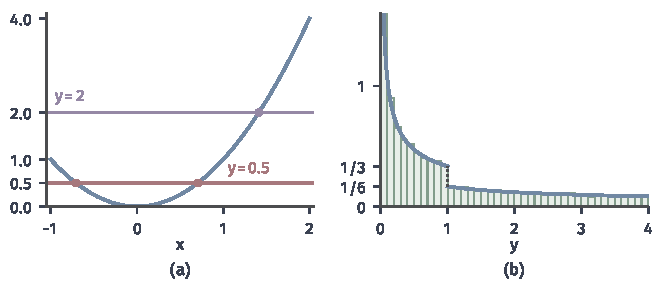
\includegraphics[width=112mm]{figures/07-probability/01-elementary-probability/matplotlib/rvt-square-branches/figure.pdf}
  \caption{多分支的平方变换，$X\sim\operatorname{Unif}(-1,2)$，$Y=X^2$。(a)蓝线是$g$在支撑上的部分，红线$y=0.5$与它有两个交点，紫线$y=2$只有一个。(b)$Y$的密度（蓝）在$y=1$处跳到一半，浅绿直方图是$20000$个模拟样本（种子$11$）。}
  \label{fig:rvt-square-branches}
\end{BookInlineFigure}

\paragraph{绝对值变换}
$Y=\lvert X\rvert$时两支是$x=y$与$x=-y$，导数的绝对值都是$1$，式~\eqref{eq:rvt-branch-density}给出
\[
 f_Y(y)=f_X(y)+f_X(-y),\qquad y>0 .
\]
左半轴的密度被对折到右半轴，与右半轴原有的密度相加。$X\sim\mathcal{N}(0,1)$时得到$f_Y(y)=2\varphi(y)$。

\paragraph{原子质量}
带原子的输入要单独处理原子。离散变量直接用式~\eqref{eq:rvt-discrete-pushforward}：$X$在$\{-2,-1,0,1,2\}$上等可能，则$\lvert X\rvert$的质量为
\[
 p_Y(0)=\frac15,\qquad p_Y(1)=\frac25,\qquad p_Y(2)=\frac25 .
\]

更常见的是混合型的输入。设$X$以概率$0.3$取$0$，以概率$0.7$按$\mathcal{N}(0,1)$取值，即
\[
 F_X(x)=0.3\cdot\mathbf{1}_{\{x\geq0\}}+0.7\,\Phi(x) .
\]
$Y=\lvert X\rvert$在$0$处的原子来自$X$在$0$处的原子，质量$0.3$；其余质量按绝对值公式对折。对$y\geq0$，
\[
 F_Y(y)=\mathbb{P}(-y\leq X\leq y)=0.3+0.7\bigl(2\Phi(y)-1\bigr) .
\]

$Y$在$(0,\infty)$上的连续部分是$0.7\cdot2\varphi(y)$，积分只有$0.7$。若只写出这个“密度”，就丢掉了$0$处的$0.3$；若把它当成完整的密度再归一化，又把原子错误地抹进了连续部分。图~\ref{fig:rvt-abs-atom}画出两个分布函数，原子表现为跳跃，在变换前后保持在$0$处。

\begin{BookInlineFigure}
  \centering
  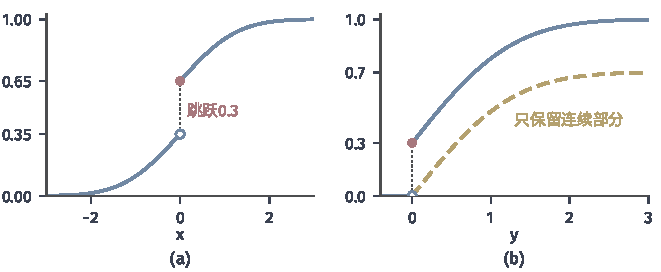
\includegraphics[width=112mm]{figures/07-probability/01-elementary-probability/matplotlib/rvt-abs-atom/figure.pdf}
  \caption{带原子的绝对值变换。(a)$X$的分布函数（蓝），在$0$处跳跃$0.3$（红点）。(b)$Y=\lvert X\rvert$的分布函数（蓝），跳跃保持在$0$；黄色虚线是只保留连续部分$0.7\cdot2\varphi$的累计，它最终只到$0.7$。}
  \label{fig:rvt-abs-atom}
\end{BookInlineFigure}

一元变换的两步做法到此可以总结为：分布函数法总是可用；需要密度时，先把输入切成单调的分支，检查每支上导数不为零，再按式~\eqref{eq:rvt-branch-density}相加；原子与导数为零的区间另算质量。
